\section{Tree-Based}


\begin{frame}[c]{Tree-based}
    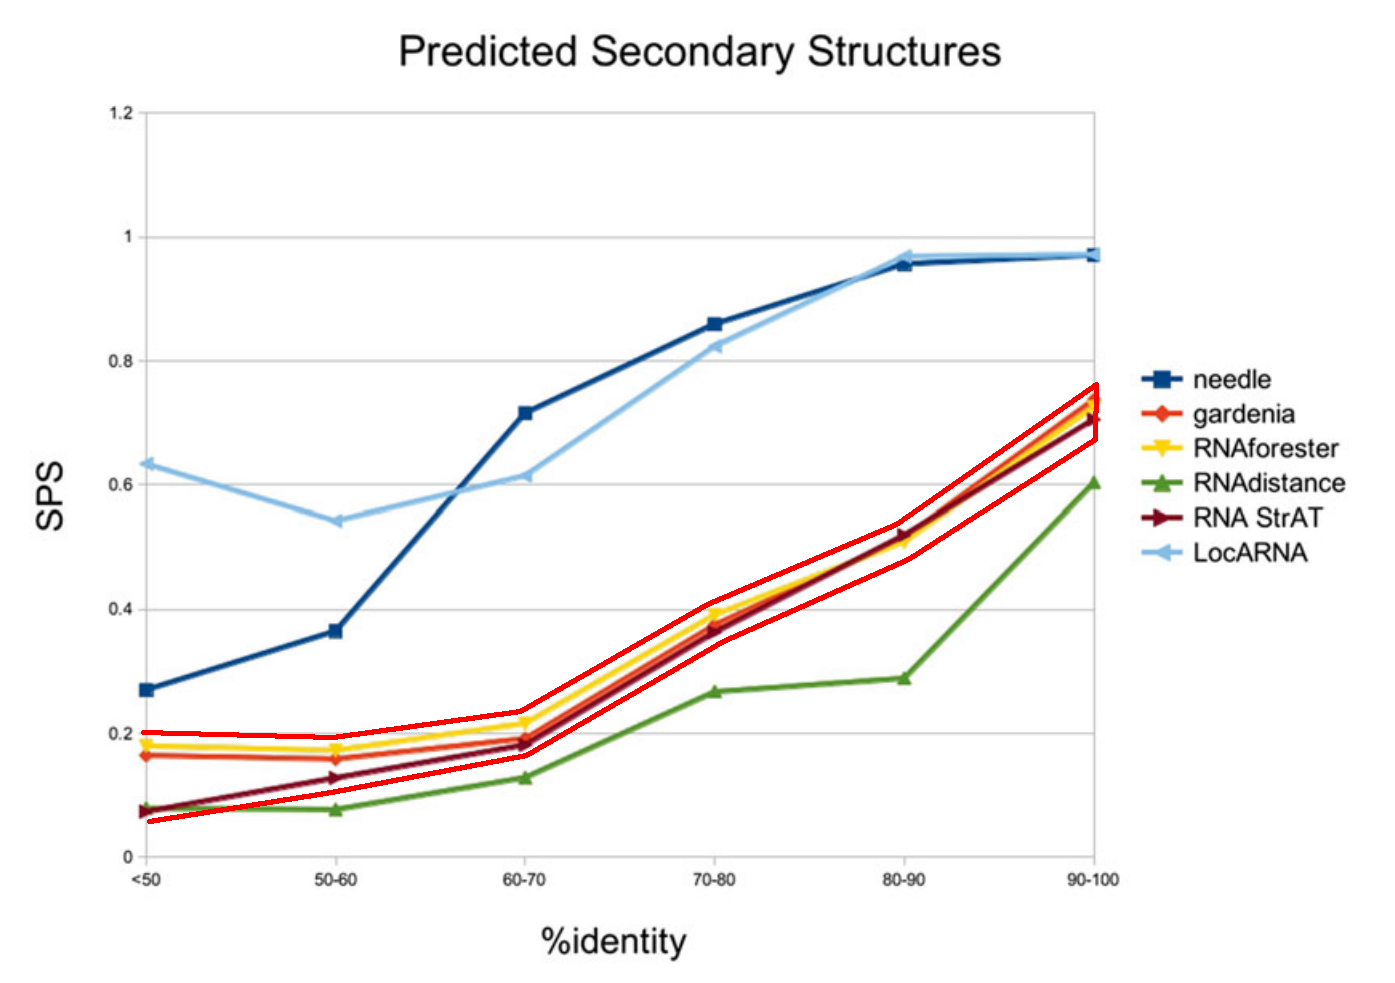
\includegraphics[width=\textwidth]{predicted_tree}
\end{frame}


\begin{frame}[c]{Tree-based}
    \Large
    Using the secondary structure:
    \newline
    \newline
    % trim = l b r t
    \begin{overprint}
    \only<2>{\centering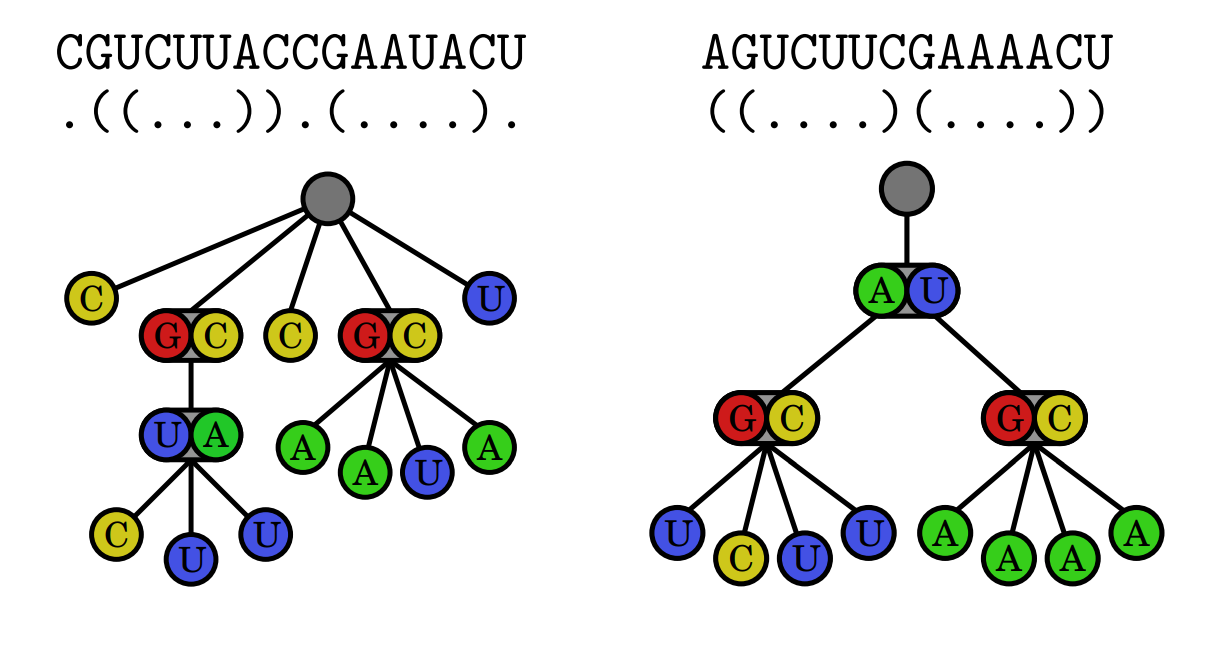
\includegraphics[width=0.47\textwidth, clip=true, trim = 0mm 0mm 230mm 0mm]{tree_sequences}}
    \only<3>{\centering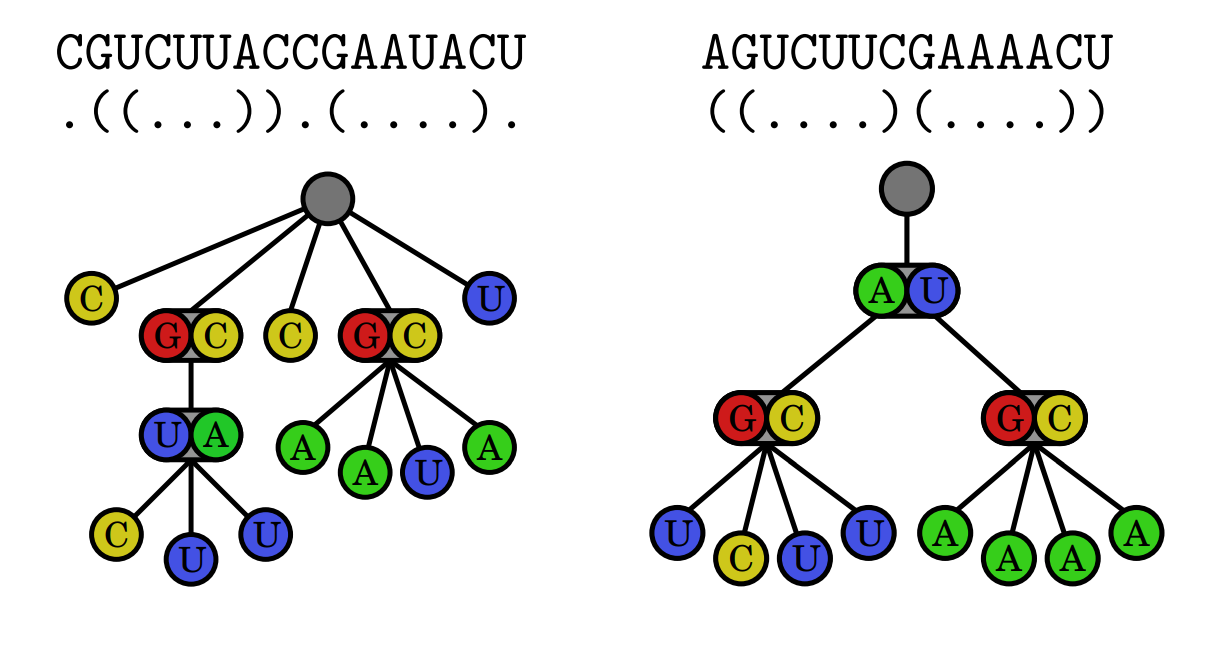
\includegraphics[width=\textwidth]{tree_sequences}}
    \end{overprint}
\end{frame}


\begin{frame}[c]{Tree-Alignment}
    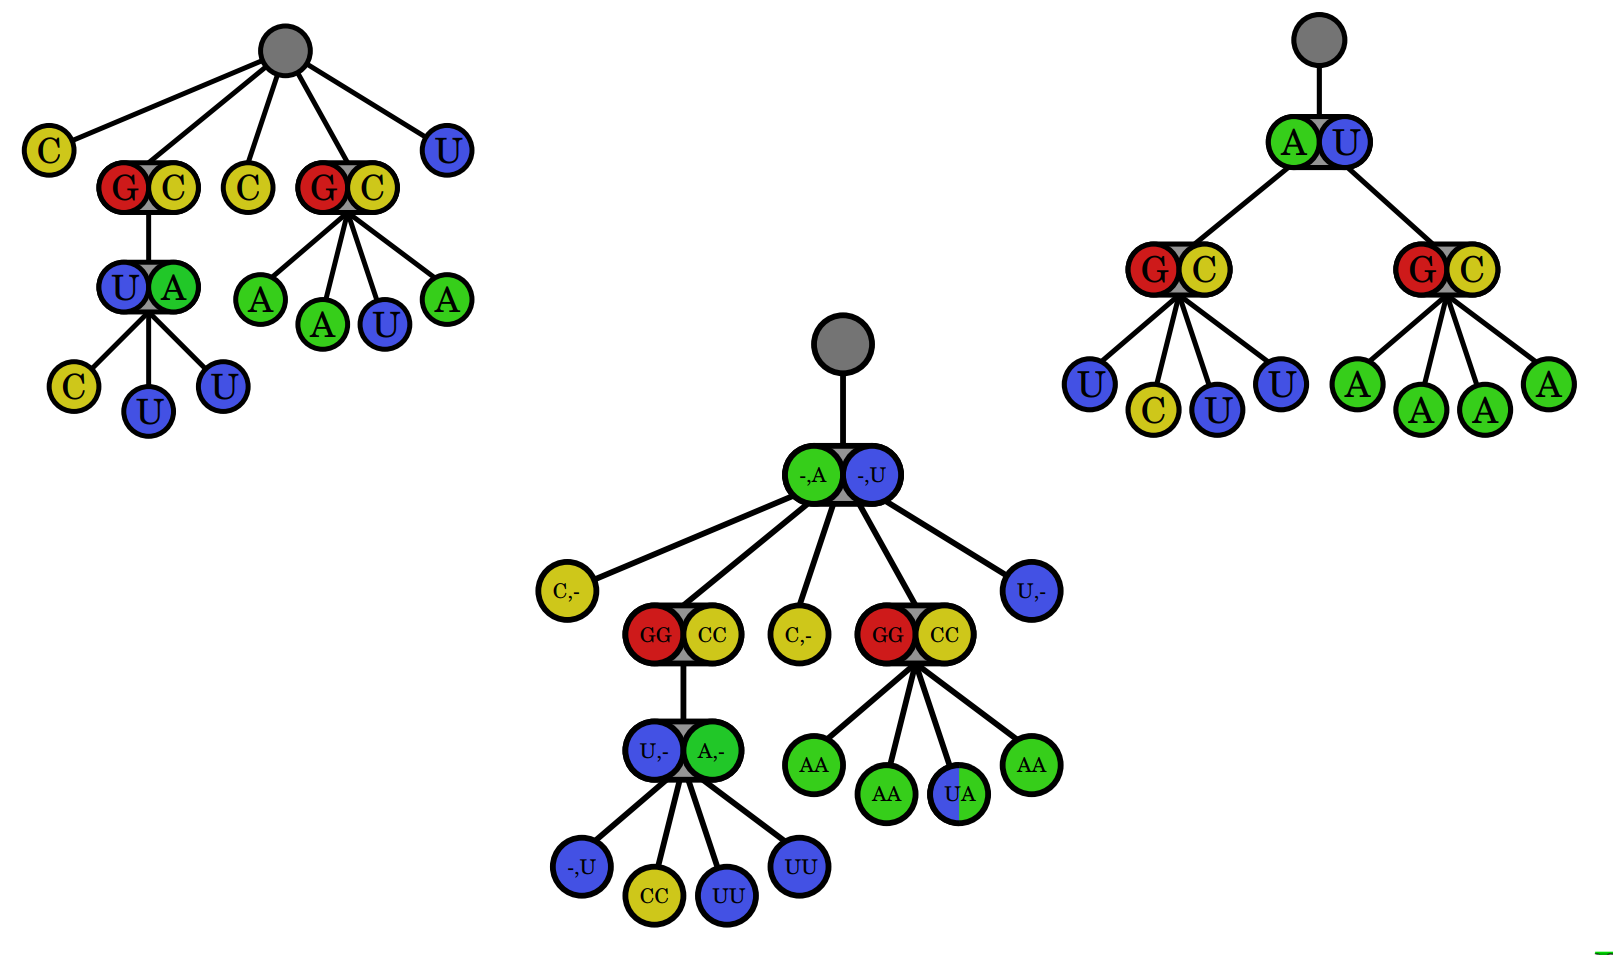
\includegraphics[width=1.03\textwidth]{tree_align}
\end{frame}

\begin{frame}[c]{Tree-Alignment Problems}
    \Large
    \begin{itemize}[<+(1)->]
        \item This is not always possible.
        \item There's structures that cannot be represented in trees.
        \newline
    \end{itemize}
    \pause
    Example: \texttt{(.[.).]}
\end{frame}



\begin{frame}[c]{Tree-Editing}
    \Large
    Edit operations on Trees ... \newline \pause
    ... are edit operations on arc-annotated sequences! \pause (\texttt{.((..(..)..))})
\end{frame}


\begin{frame}[c]{Tree-Editing Possibilities}
    % 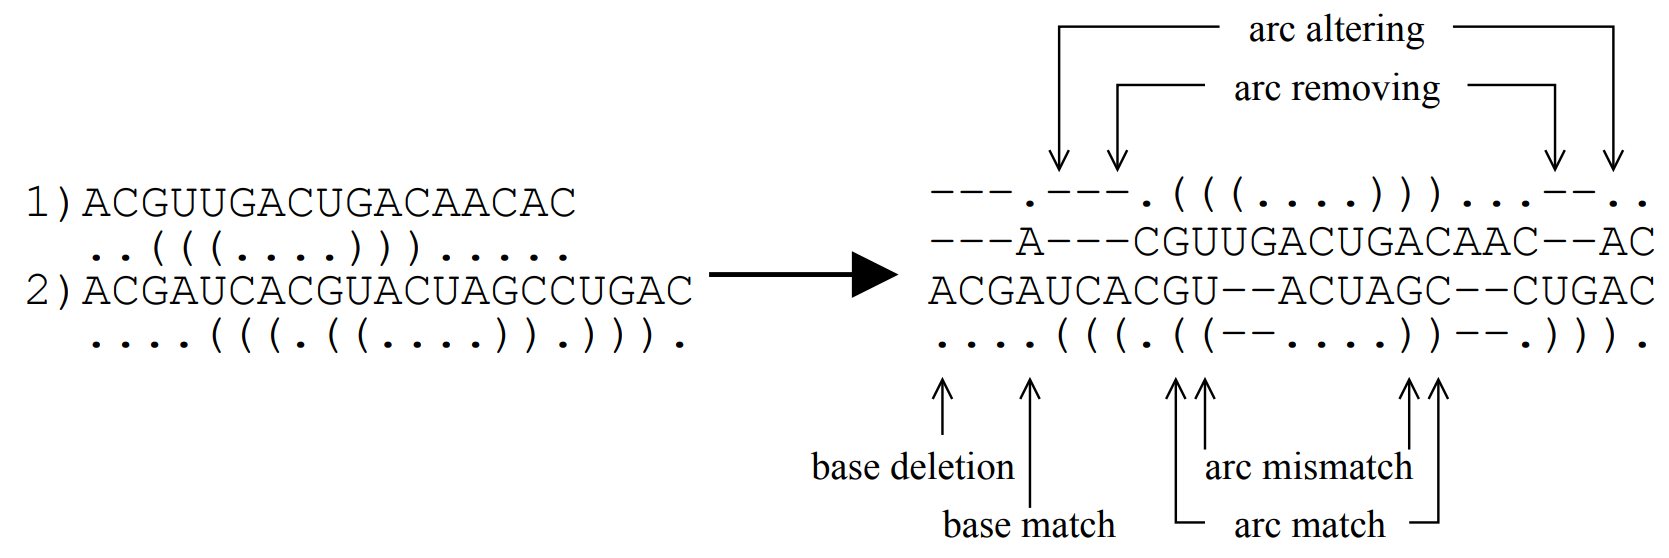
\includegraphics[width=\textwidth]{arc_things}
    \hspace{0mm}
    \begin{overprint}
    \onslide<1>\centering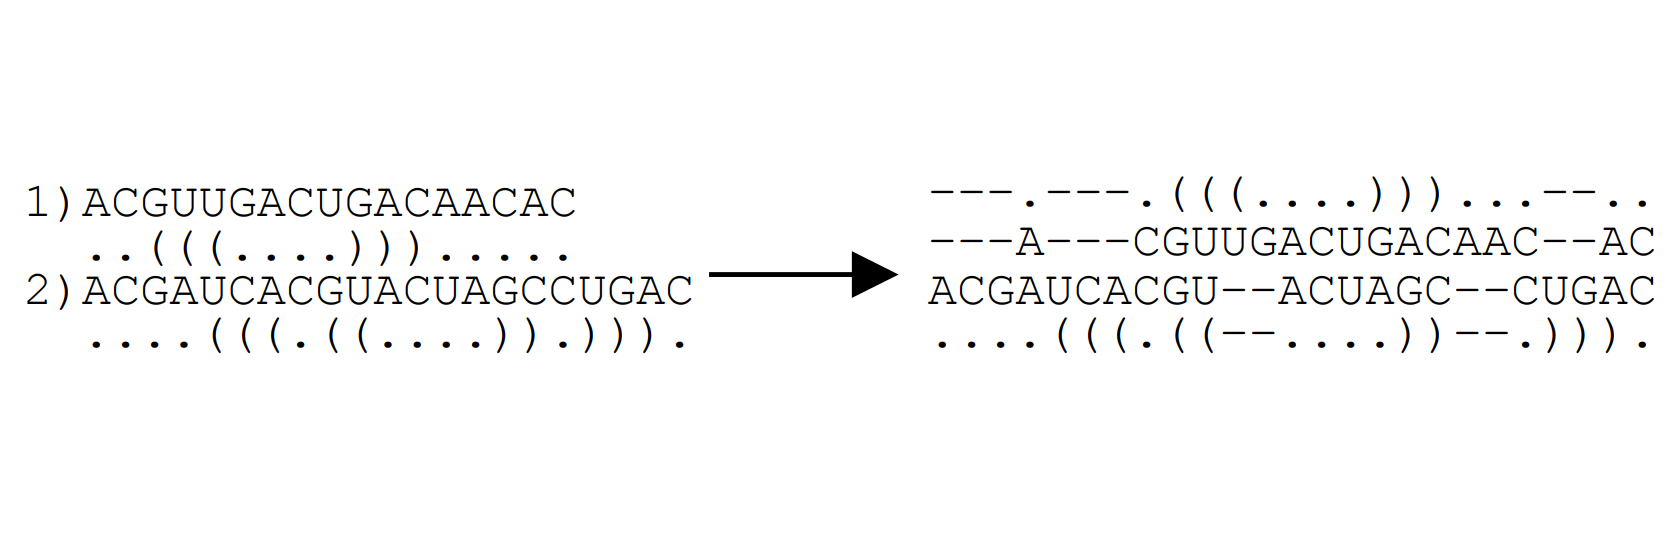
\includegraphics[width=\textwidth]{arc_example}
    \onslide<2>\centering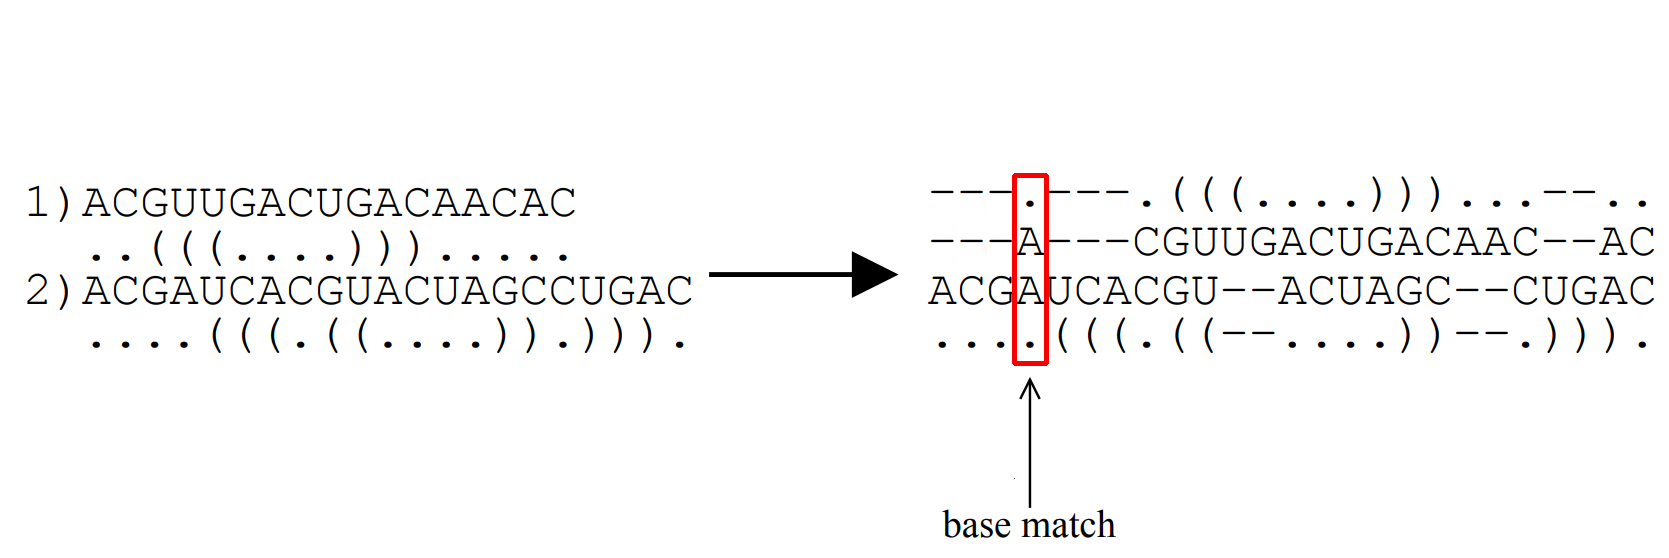
\includegraphics[width=\textwidth]{base_match}
    \onslide<3>\centering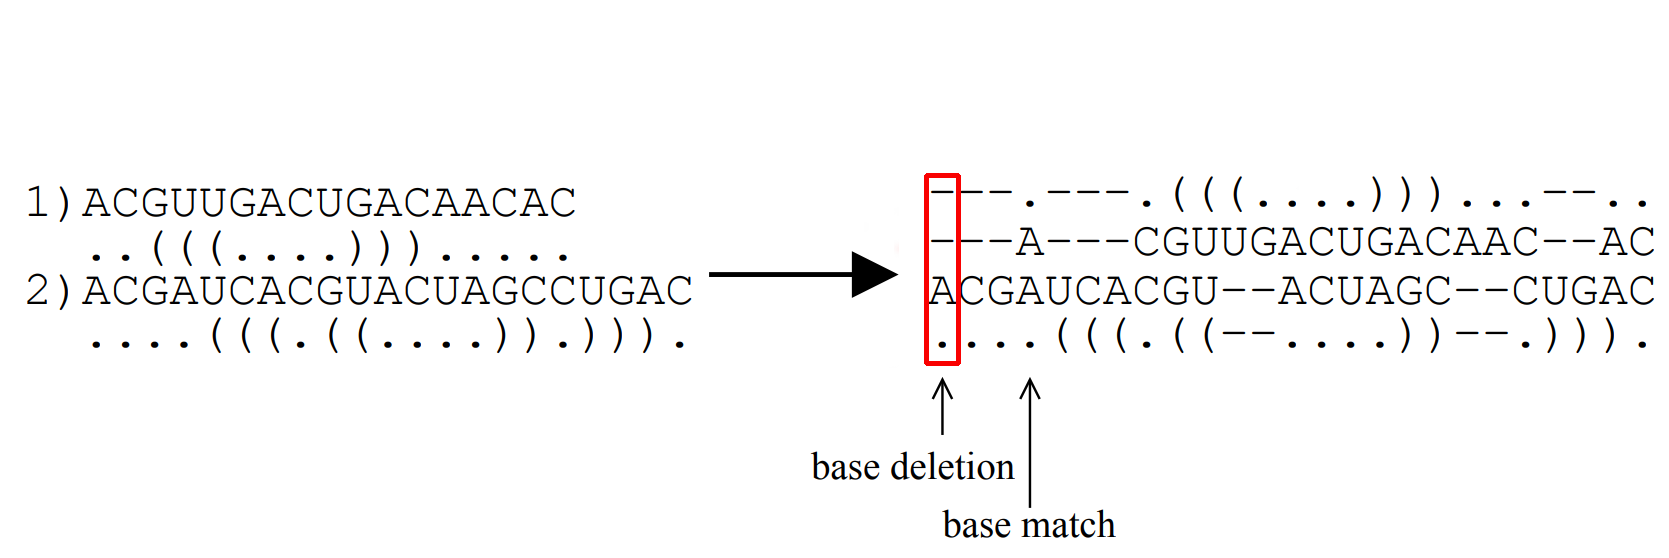
\includegraphics[width=\textwidth]{base_indel}
    \onslide<4>\centering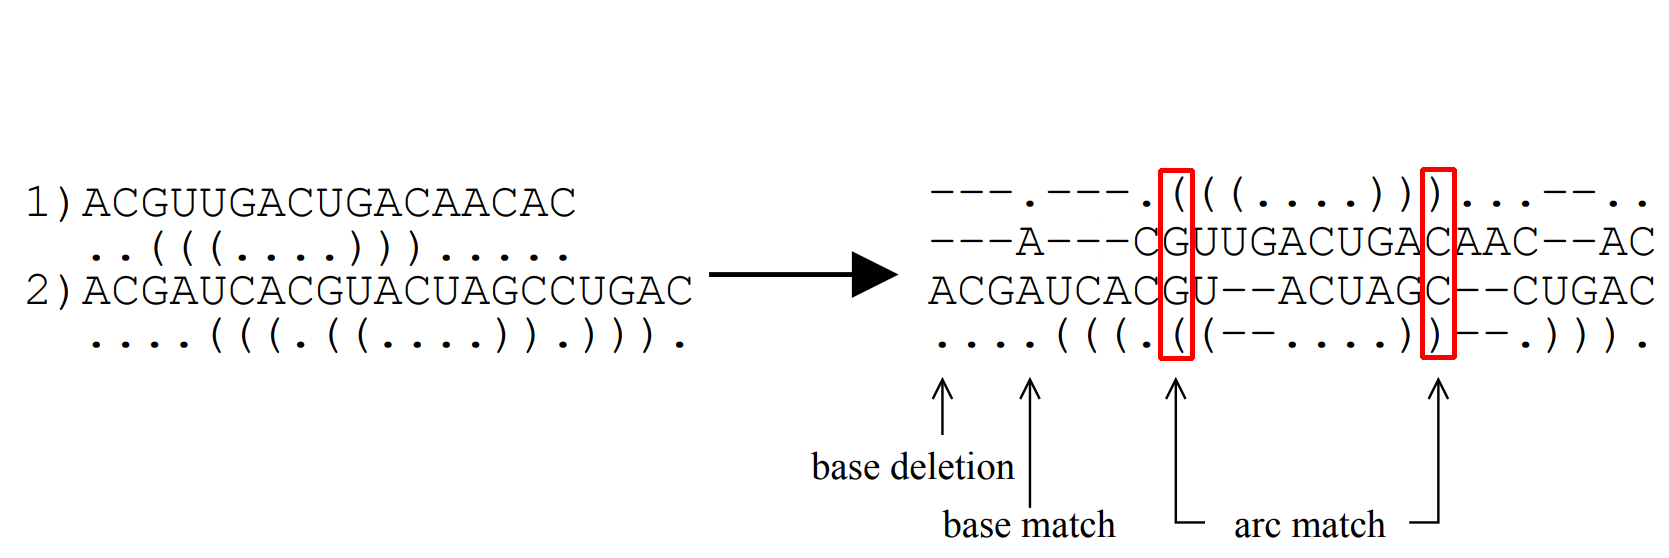
\includegraphics[width=\textwidth]{arc_match}
    \onslide<5>\centering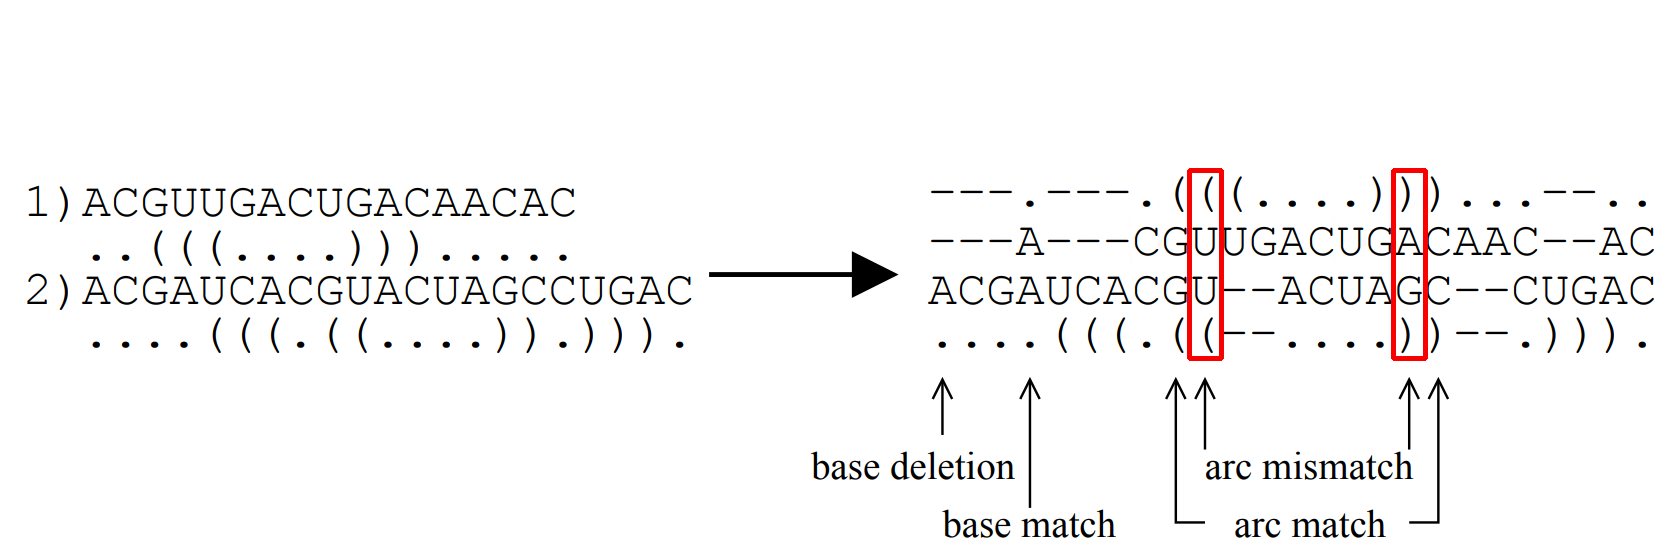
\includegraphics[width=\textwidth]{arc_mismatch}
    \onslide<6>\centering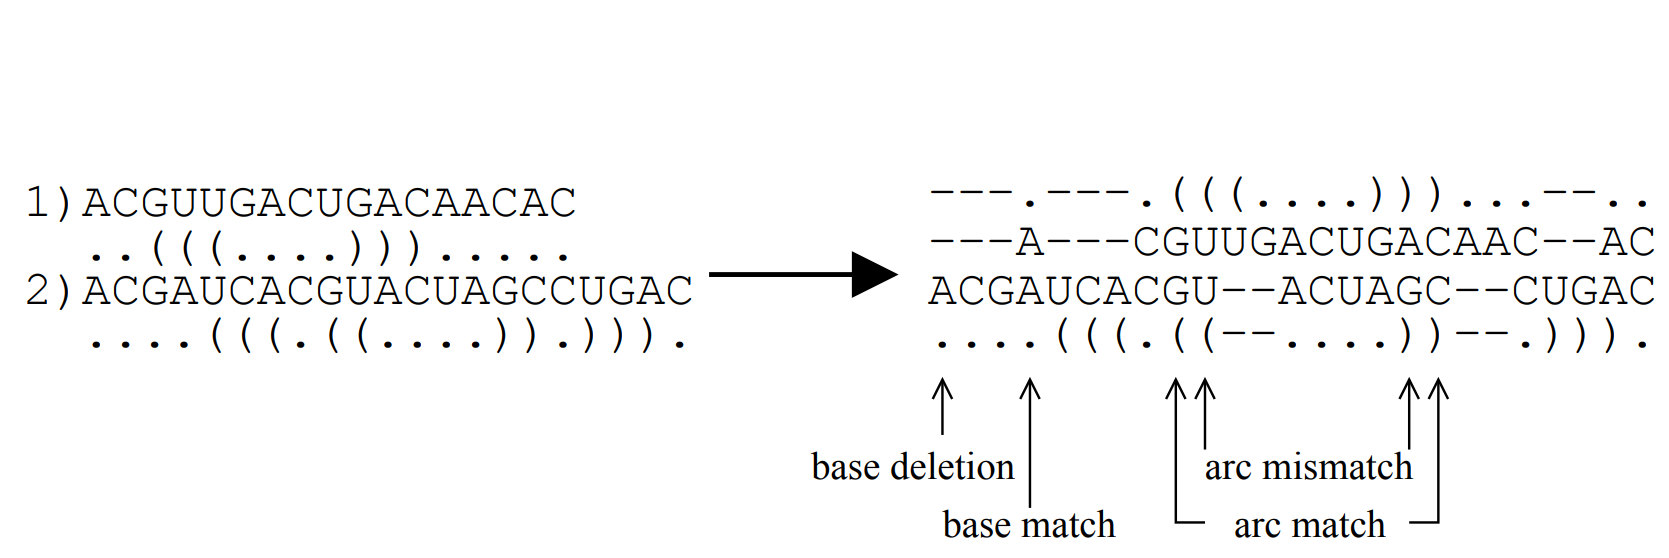
\includegraphics[width=\textwidth]{arc_breaking}
    \onslide<7>\centering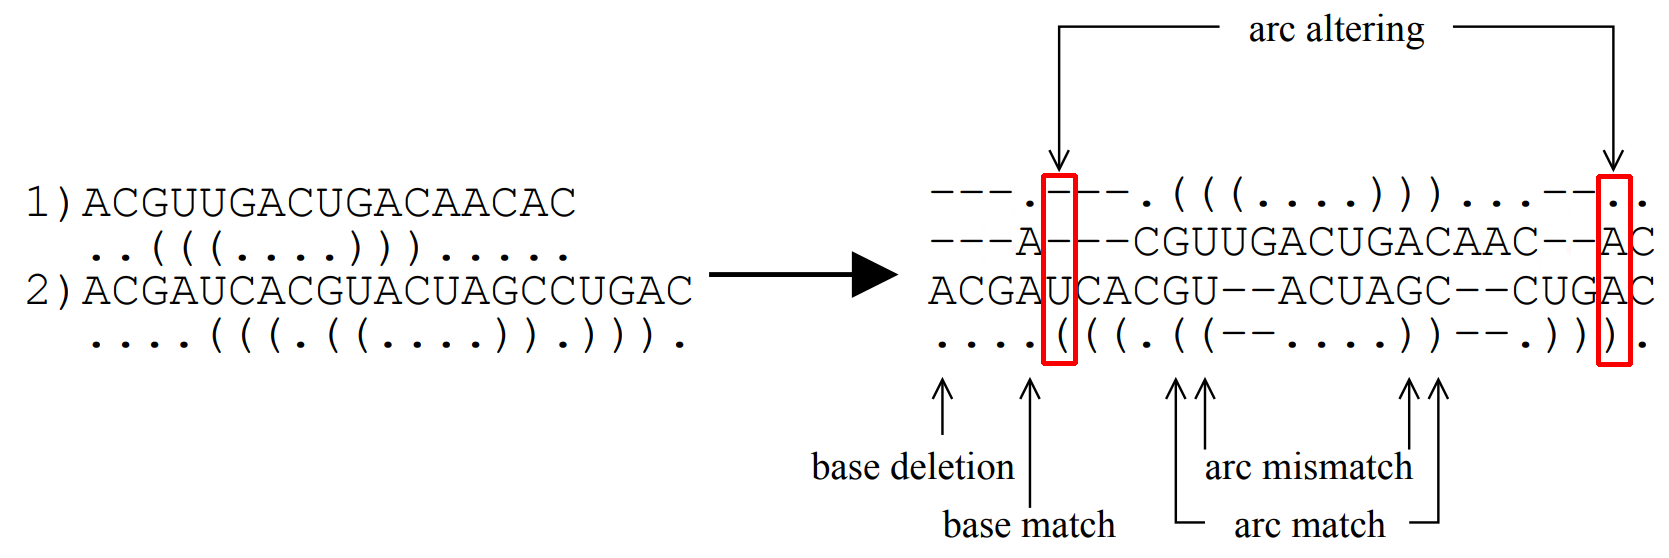
\includegraphics[width=\textwidth]{arc_altering}
    \onslide<8>\centering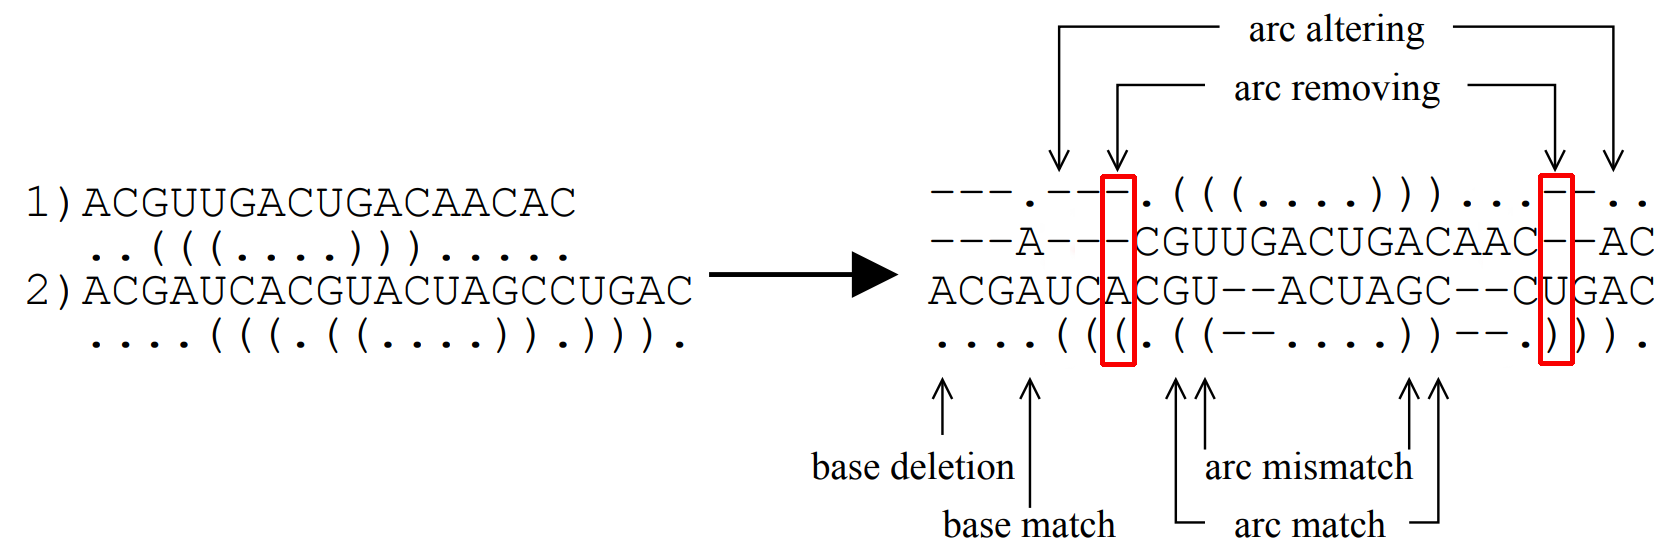
\includegraphics[width=\textwidth]{arc_removing}
    \end{overprint}

    \begin{multicols}{2}
    \begin{itemize}[<+(1)->]
        \item base match
        \item base indel
        \item arc match
            % arc on both strands match!
        \item arc mismatch
            % there is an arc on both, but there's different base pairs!
        \item arc breaking (missing)
            % there is an arc in one, but not in the other. Same bases though.
        \item arc altering
            % in one there's an arc, in the other only one of the two bases
        \item arc removing
            % there's nothing to resemble the arc in the other strand
    \end{itemize}
    \end{multicols}
\end{frame}

\begin{frame}[c]{Performance comparison}
    \hspace{0mm}
    \begin{overprint}
    \onslide<1>\centering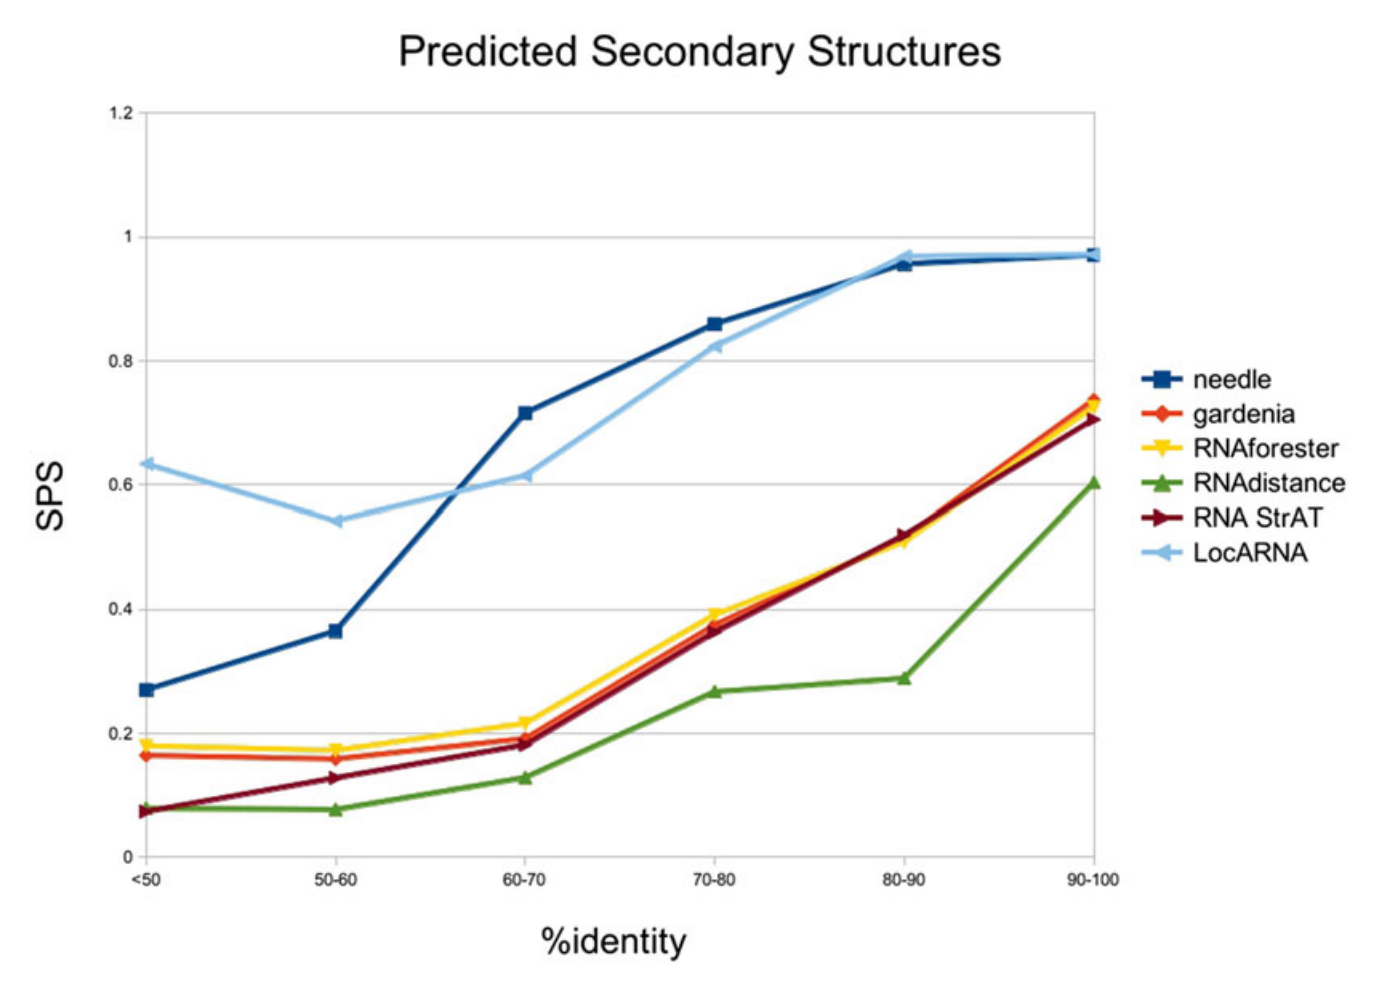
\includegraphics[width=0.9\textwidth]{predicted}
    \onslide<2>\centering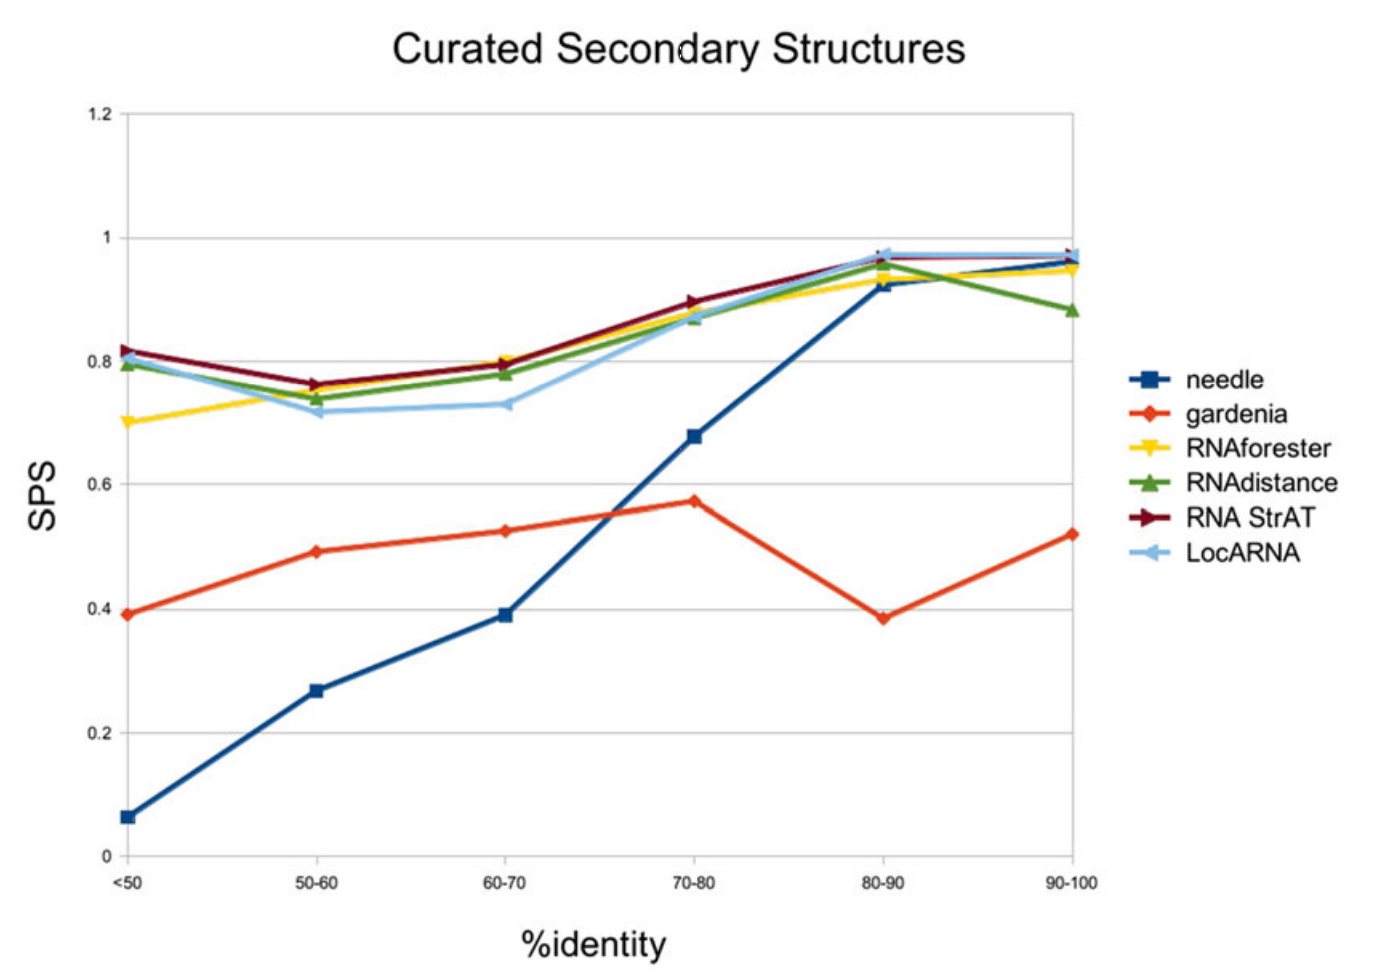
\includegraphics[width=0.9\textwidth]{curated}
    \end{overprint}
\end{frame}


\begin{frame}[c]{Tree-based Alignment}
    \Large
    \pause
    Basically a structure-using edit distance.
\end{frame}

